\section{Implementação Serial}

\subsection{Implementação em Java}

\subsubsection{Descrição}

A implementação serial em Java é composta por quatro classes principais, cada uma
com responsabilidade bem delimitada:

\begin{itemize}
    \item \texttt{CsvDataset} — lê o cabeçalho do arquivo CSV e expõe os dados
          linha a linha via \texttt{forEachPoint}, sem carregar o dataset inteiro
          em memória;
    \item \texttt{KMeans} — contém o algoritmo K-Means: inicialização dos
          centróides, laço de atribuição e recomputo, verificação de convergência
          e avaliação final;
    \item \texttt{KMeansResult} — registro imutável que armazena os centróides
          finais, tamanhos de cluster, número de iterações e soma dos erros
          quadráticos;
    \item \texttt{Main} — ponto de entrada; configura \(k = 10\),
          \texttt{maxIter} = 10 e \texttt{tolerance} = \(10^{-6}\) e imprime o
          resumo dos clusters ao final.
\end{itemize}

\begin{figure}[H]
  \centering
  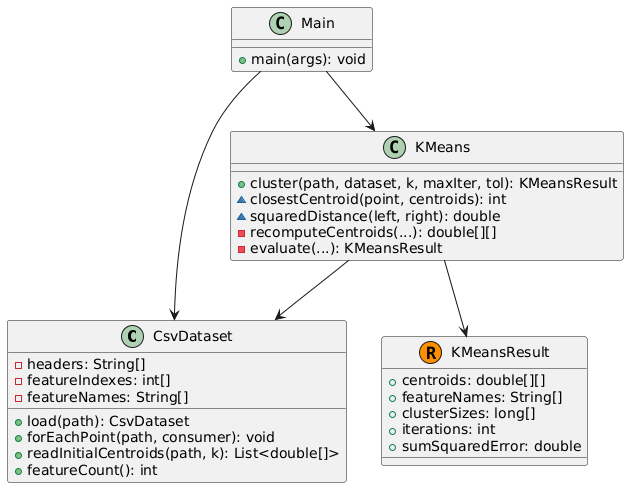
\includegraphics[width=0.6\textwidth]{img/3-serial/class-diagram}
  \caption{Diagrama de classes da implementação serial em Java.}
  \label{fig:class-diagram-serial-java}
\end{figure}

O dataset é processado em modo \textit{streaming}: a cada iteração do algoritmo,
\texttt{forEachPoint} abre o arquivo, lê e descarta o cabeçalho, e entrega cada
linha decodificada ao consumidor sem acumular pontos na memória heap. A
Figura~\ref{fig:snippet-foreach} mostra essa interface.

\begin{figure}[H]
    \centering
    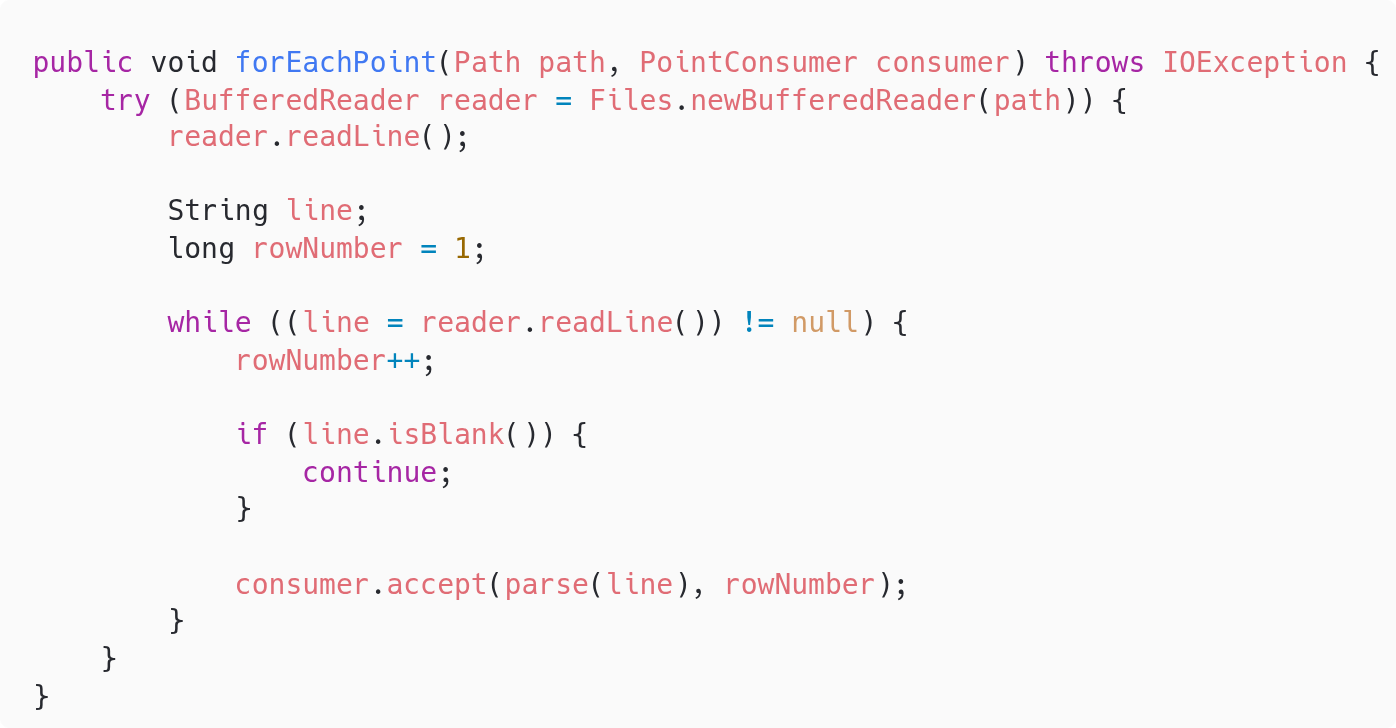
\includegraphics[width=0.85\textwidth]{img/3-serial/snippet-1}
    \caption{Leitura linha a linha do dataset (\texttt{CsvDataset.forEachPoint}).}
    \label{fig:snippet-foreach}
\end{figure}

O laço principal do algoritmo, mostrado na Figura~\ref{fig:snippet-cluster-loop},
percorre todos os pontos a cada iteração para acumular somas parciais e contagens
por cluster, e em seguida recomputa os centróides dividindo as somas pelas
contagens.

\begin{figure}[H]
    \centering
    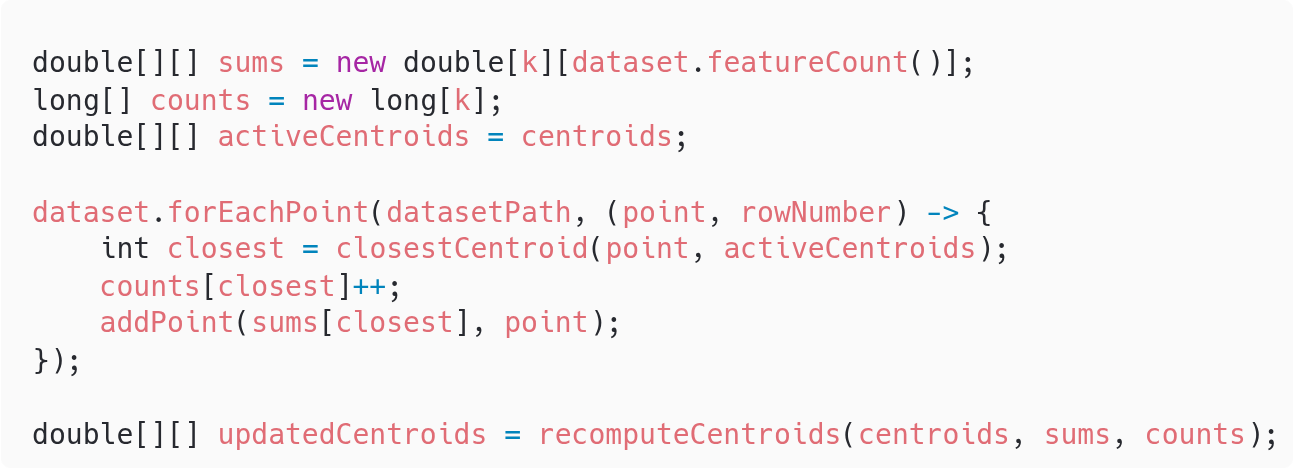
\includegraphics[width=0.85\textwidth]{img/3-serial/snippet-2}
    \caption{Laço de atribuição e recomputo de centróides (\texttt{KMeans.cluster}).}
    \label{fig:snippet-cluster-loop}
\end{figure}

A função \texttt{closestCentroid} (Figura~\ref{fig:snippet-closest}) varre os \(k\)
centróides para cada ponto e retorna o índice do mais próximo usando distância
euclidiana ao quadrado, evitando a raiz quadrada desnecessária. Essa função é
o principal ponto quente da CPU, executada \(N \times k\) vezes por iteração.

\begin{figure}[H]
    \centering
    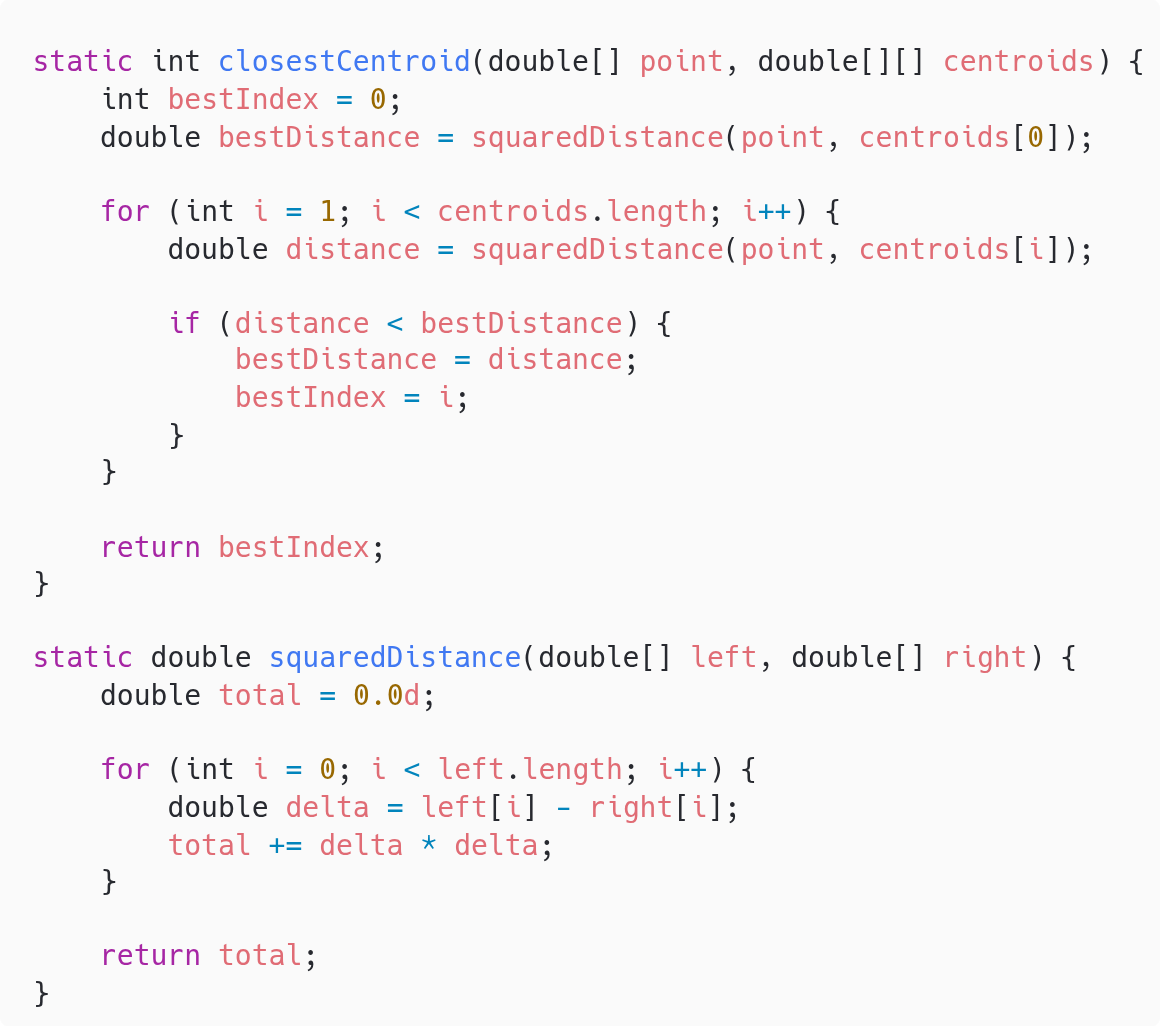
\includegraphics[width=0.85\textwidth]{img/3-serial/snippet-3}
    \caption{Busca do centróide mais próximo e distância euclidiana ao quadrado.}
    \label{fig:snippet-closest}
\end{figure}

\subsubsection{Resultados}

\paragraph{Avaliação com Microbenchmark}

Os microbenchmarks foram executados com JMH 1.37 sobre JDK 25.0.1 (OpenJDK 64-Bit
Server VM), com 1 fork, 1 iteração de aquecimento de 10 s e 3 iterações de medição
de 10 s cada. O dataset utilizado possui aproximadamente 1 GB de dados de pedidos
sintéticos.

\begin{table}[h]
\centering
\begin{tabular}{llrrr}
\hline
\textbf{ID} & \textbf{Benchmark} & \textbf{Média} & \textbf{Erro ($\pm$)} & \textbf{Unidade} \\
\hline
B1 & Execução completa (\textit{k}=10, maxIter=20) & 212{,}57 & 34{,}48 & s/op \\
B2 & Custo por iteração (\textit{k}=10, maxIter=5)  &  60{,}05 &  2{,}46 & s/op \\
B3 & \texttt{closestCentroid} (\textit{k}=10, 38 dims) &  96{,}82 &  5{,}59 & ns/op \\
B4 & \texttt{squaredDistance} (38 dims)               &   9{,}31 &  1{,}41 & ns/op \\
\hline
\end{tabular}
\caption{Resultados JMH para a implementação serial em Java.}
\label{tab:jmh-serial-java}
\end{table}

B2 mostra que cada iteração leva cerca de 12 s, dominado pela releitura do CSV a cada
ciclo. B3 e B4 mostram que o cálculo aritmético é rápido (96 ns e 9 ns por chamada).
O gargalo não está na CPU, mas na leitura e no parsing do arquivo.

% Mostrar tabela de resultados comparando Java com a linguagem escolhida

\paragraph{Avaliação com Macrobenchmark}

Os macrobenchmarks foram executados com JMeter 5.6.3 sobre JDK 25.0.1, com
\(k = 10\), \texttt{maxIter} = 3 e \texttt{tol} = 0,0. Cada configuração
(GC $\times$ threads) rodou por 120 s com ramp-up de 30 s. A
Tabela~\ref{tab:jmeter-serial-java} apresenta a throughput obtida em cada combinação.

\begin{table}[H]
\centering
\begin{tabular}{rrrrr}
\hline
\textbf{Threads} & \textbf{G1GC} & \textbf{ZGC} & \textbf{ParallelGC} & \textbf{Unidade} \\
\hline
1  & 1,56 & 1,50 & 1,52 & execuções/min \\
2  & 2,25 & 2,01 & 2,26 & execuções/min \\
4  & 2,70 & 2,54 & 2,79 & execuções/min \\
8  & 3,44 & 3,23 & 3,51 & execuções/min \\
16 & 4,66 & 4,40 & 4,85 & execuções/min \\
\hline
\end{tabular}
\caption{Throughput por número de threads e coletor de GC --- implementação serial em Java.}
\label{tab:jmeter-serial-java}
\end{table}

O throughput cresce com o número de threads JMeter, mas com retornos decrescentes:
de 1 para 16 threads, o ganho é de $\approx$3$\times$. A latência piora com mais
threads, pois todas as instâncias leem o mesmo arquivo de $\approx$1 GB ao mesmo
tempo, saturando a I/O do disco.

\paragraph{Avaliação de Profile}

O profile foi capturado com JFR (\texttt{settings=profile}) sobre uma execução completa
do algoritmo serial (\(k=10\), \texttt{maxIter=3}, G1GC, dataset $\approx$1 GB).
A gravação durou 118 s e foi analisada com a ferramenta \texttt{jfr} do JDK 25.

\textbf{Hot Methods.}
A Tabela~\ref{tab:jfr-hot-methods} apresenta os métodos com maior frequência de
amostragem de CPU (\texttt{jdk.ExecutionSample}, 11.054 amostras no total).

\begin{table}[H]
\centering
\begin{tabular}{lrrl}
\hline
\textbf{Método} & \textbf{Amostras} & \textbf{CPU (\%)} & \textbf{Categoria} \\
\hline
\texttt{FloatingDecimal.readJavaFormatString} & 2784 & 25,2 & Parsing CSV \\
\texttt{String.split}                         & 1873 & 16,9 & Parsing CSV \\
\texttt{FloatingDecimal.copyDigits}           & 1817 & 16,4 & Parsing CSV \\
\texttt{FloatingDecimal.parseDouble}          & 1782 & 16,1 & Parsing CSV \\
\texttt{FloatingDecimal.doubleValue}          &  831 &  7,5 & Parsing CSV \\
\texttt{KMeans.squaredDistance}               &  638 &  5,8 & Algoritmo   \\
\texttt{BufferedReader.readLine}              &  609 &  5,5 & I/O         \\
\texttt{KMeans.closestCentroid}               &  205 &  1,9 & Algoritmo   \\
\texttt{KMeans.addPoint}                      &   33 &  0,3 & Algoritmo   \\
\hline
\end{tabular}
\caption{Hot methods na implementação serial em Java (JFR, 11.054 amostras).}
\label{tab:jfr-hot-methods}
\end{table}

O parsing CSV (\texttt{String.split} + \texttt{Double.parseDouble} e suas
dependências internas) consome $\approx$82\% do tempo de CPU, revelando que o
gargalo real não é a leitura de disco em si, mas a conversão de texto para
\texttt{double} linha a linha. O código aritmético do K-Means
(\texttt{squaredDistance} + \texttt{closestCentroid} + \texttt{addPoint})
representa apenas $\approx$8\% — coerente com os resultados JMH de B3 (96 ns/op)
e B4 (9 ns/op).

\textbf{GC.}
Foram realizadas 1.099 coletas Young GC em 118 s (9,3/s), com pausa total de
805 ms — apenas 0,68\% do tempo de execução. O heap oscila entre
$\approx$150 MB e $\approx$5 MB após cada coleta, reflexo da alta taxa de
criação e descarte de objetos \texttt{String} durante o parsing. O GC não é
um gargalo.

\textbf{Threads.}
Uma única thread de trabalho executa todo o algoritmo; as demais 7 threads
são internas da JVM (GC, compilador JIT, etc.). Não há contenção nem
paralelismo.

\textbf{Síntese.}
O principal gargalo é o parsing CSV (\texttt{String.split} + \texttt{Double.parseDouble}),
que consome $\approx$82\% do CPU. O cálculo aritmético do K-Means representa apenas $\approx$8\%.

\iffalse % ============================================================
% ERLANG — seção desativada, manter para uso futuro
\subsection{\sout{Implementação em Erlang}}

\subsubsection{\sout{Descrição}}

% Descrever como o algoritmo foi implementado na outra linguagem

\subsubsection{\sout{Resultados}}

\paragraph{\sout{Avaliação com Microbenchmark}}

\paragraph{\sout{Avaliação com Macrobenchmark}}

\paragraph{\sout{Avaliação de Profile}}
\fi % ============================================================

\subsection{Discussão}

\textbf{Trechos caros e candidatos à concorrência.}
O JFR mostra que $\approx$82\% do CPU é gasto com parsing CSV
(\texttt{String.split} + \texttt{Double.parseDouble}). O laço de atribuição,
que chama \texttt{closestCentroid} $N \times k$ vezes por iteração, é
independente entre pontos e é o principal candidato à paralelização. A
releitura do arquivo a cada iteração (\texttt{forEachPoint}) é outro gargalo
que poderia ser eliminado carregando o dataset em memória.

\textbf{Comparação de coletores de GC.}
A Tabela~\ref{tab:jmeter-serial-gc} compara o throughput por coletor em três
níveis de carga.

\begin{table}[H]
\centering
\begin{tabular}{lrrrr}
\hline
\textbf{GC} & \textbf{1 thread} & \textbf{4 threads} & \textbf{16 threads} & \textbf{Unidade} \\
\hline
G1GC       & 1{,}56 & 2{,}70 & 4{,}66 & execuções/min \\
ZGC        & 1{,}50 & 2{,}54 & 4{,}40 & execuções/min \\
ParallelGC & 1{,}52 & 2{,}79 & 4{,}85 & execuções/min \\
\hline
\end{tabular}
\caption{Throughput por coletor de GC --- implementação serial.}
\label{tab:jmeter-serial-gc}
\end{table}

O ParallelGC tem o maior throughput em todos os níveis, seguido pelo G1GC. O ZGC
fica levemente atrás: mesmo com baixa pressão de heap, as barreiras de escrita do
seu algoritmo adicionam custo. No geral, o impacto do GC é pequeno --- as pausas
somam menos de 1\% do tempo total.
